\section{Автоматизированная сборка и тестирование}
Спустя некоторое время мне понадобилось автоматически собирать инсталляторы для каждого коммита, чтобы не тратить каждый раз время на полноценную сборку инсталлятора и deb-пакета для приложения. Для этих целей я выбрал Azure DevOps, который предоставлял бесплатные сборочные машины и целую готовую инфраструктуру для автоматизированной сборки и тестирования.\\
Для целей автоматизированного тестирования был создан интерфейс командной строки, который позволяет использовать все возможности приложения без необходимости запускать графический интерфейс пользователя, что позволило тестировать приложения в операционных системах без графической среды пользователя.\\
Сборочная цепочка для AzureDevops под операционную систему Linux на базе Ubuntu 16.04 имеет следующий вид:
\begin{figure}[H]
	\centering
	\includegraphics[width=1\linewidth]{pics/AzurePipeline.PNG}
	\caption{Azure Pipeline}
	\label{fig:AzurePipeline}
\end{figure}

В шаге Install Prereqs происходит установка QT для возможности сборки приложения.\\
Prepare Sources заменяет версию в Файле appinfo.h на текущую версию приложения, т.е. имеет вид 0.8.3.$(buildNumber)\\
Шаг Build осуществляет сборку бинарного файла приложения\\
Шаг Pack собирает Deb пакет (TODO: реализовать этот шаг)\\
Шаг GitHub Release публикует PreRelease версию на GitHub с указанием тага текущей сборки\\
\begin{figure}[H]
	\centering
	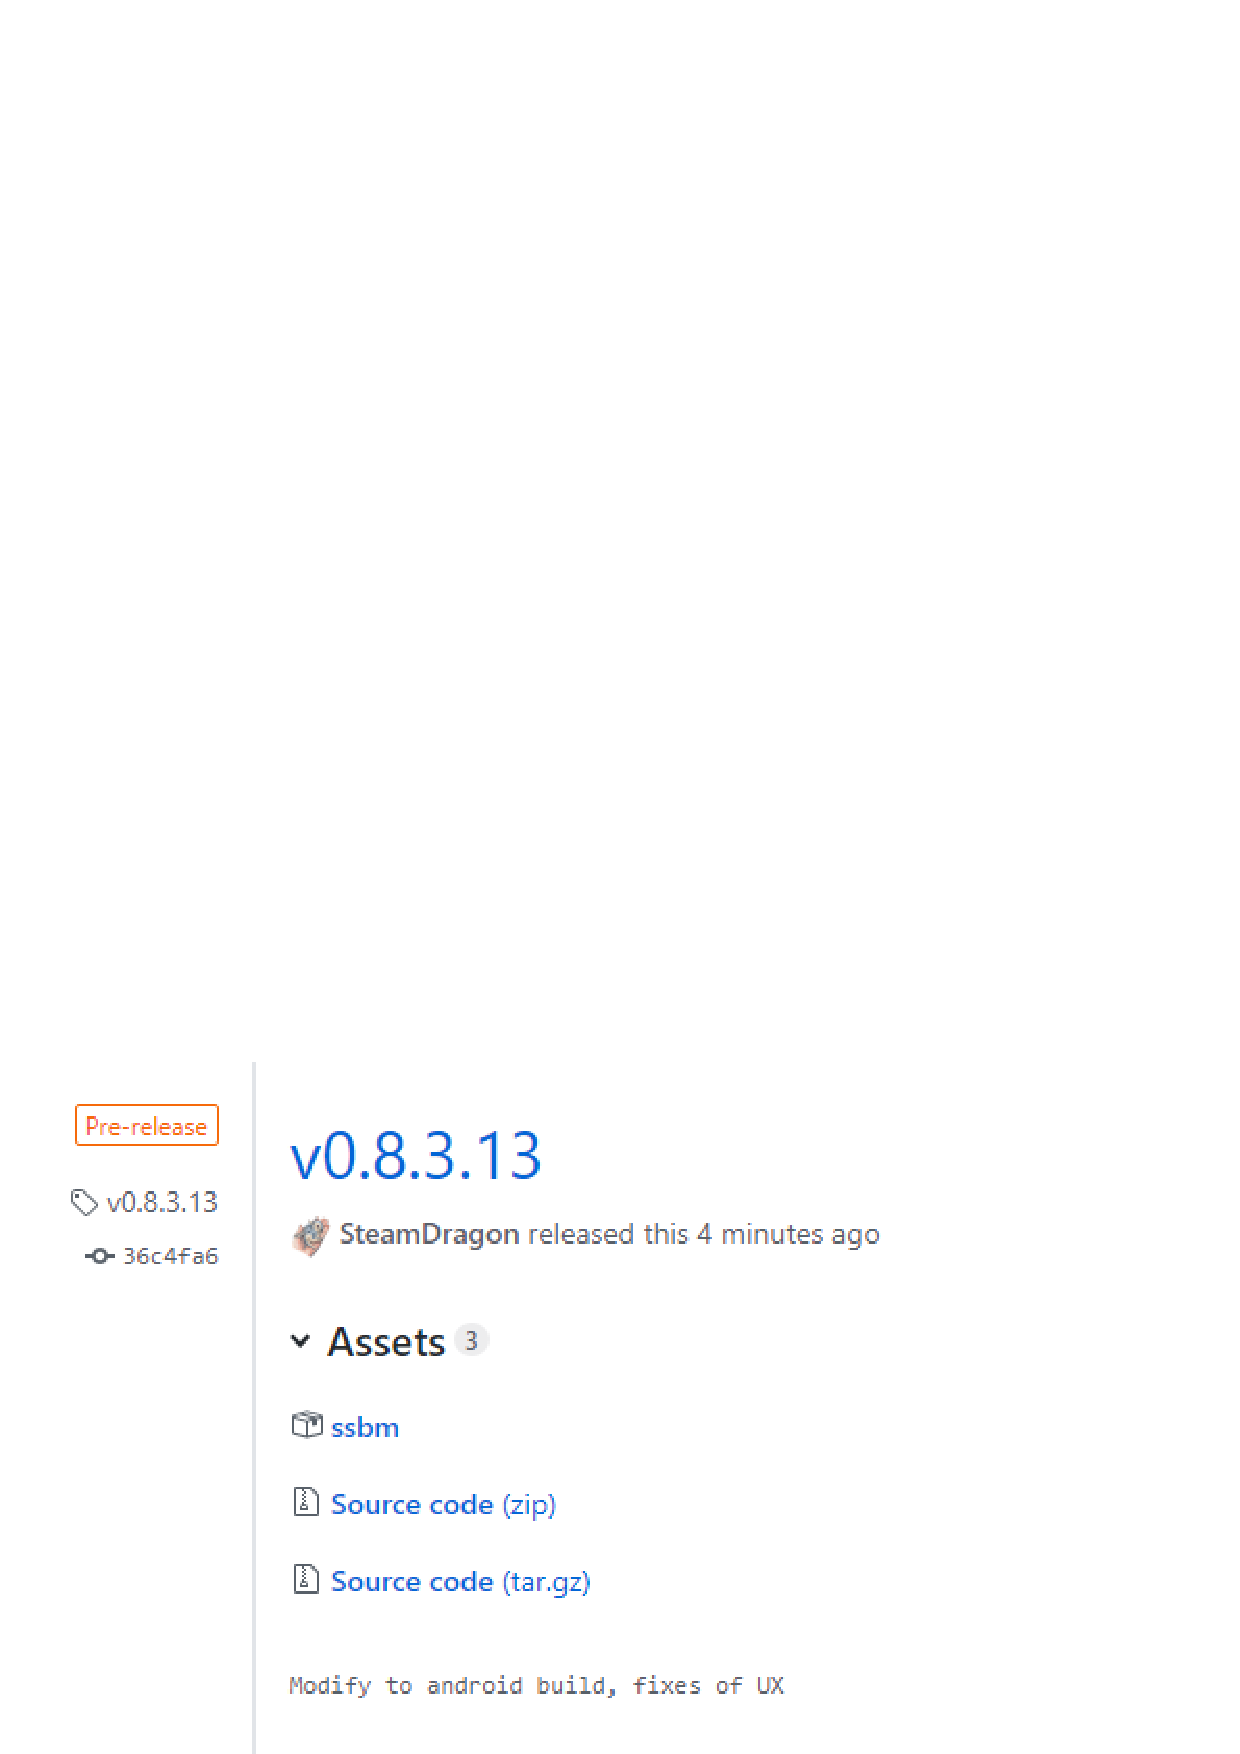
\includegraphics[width=1\linewidth]{pics/GHRelease.PNG}
	\caption{Github Release}
	\label{fig:GHRelease}
\end{figure}